\documentclass{article}
\usepackage{amsmath,amsfonts,amsthm,amssymb,amsopn,bm}
\usepackage[margin=.9in]{geometry}
\usepackage{graphicx}
\usepackage{url}
\usepackage[usenames,dvipsnames]{color}
\usepackage{fancyhdr}
\usepackage{multirow}
\usepackage{listings}
\usepackage{hyperref}

\definecolor{keywords}{RGB}{255,0,90}
\definecolor{comments}{RGB}{0,0,113}
\definecolor{red}{RGB}{160,0,0}
\definecolor{green}{RGB}{0,150,0}
 
\lstset{language=Python, 
        basicstyle=\ttfamily\tiny, 
        keywordstyle=\color{keywords},
        commentstyle=\color{comments},
        stringstyle=\color{red},
        showstringspaces=false}

\newcommand{\field}[1]{\mathbb{#1}}
\newcommand{\1}{\mathbf{1}}
\newcommand{\E}{\mathbb{E}} 
\newcommand{\Z}{\mathbb{Z}} 
\renewcommand{\P}{\mathbb{P}}
\newcommand{\R}{\field{R}} % real domain
% \newcommand{\C}{\field{C}} % complex domain
\newcommand{\F}{\field{F}} % functional domain
\newcommand{\T}{^{\textrm T}} % transpose
\def\diag{\text{diag}}

%% operator in linear algebra, functional analysis
\newcommand{\inner}[2]{#1\cdot #2}
\newcommand{\norm}[1]{\left\|#1\right\|}
\newcommand{\twonorm}[1]{\|#1\|_2^2}
% operator in functios, maps such as M: domain1 --> domain 2
\newcommand{\Map}[1]{\mathcal{#1}}
\renewcommand{\theenumi}{\alph{enumi}} 

\newcommand{\Perp}{\perp \! \! \! \perp}

\newcommand\independent{\protect\mathpalette{\protect\independenT}{\perp}}
\def\independenT#1#2{\mathrel{\rlap{$#1#2$}\mkern2mu{#1#2}}}
\newcommand{\vct}[1]{\boldsymbol{#1}} % vector
\newcommand{\mat}[1]{\boldsymbol{#1}} % matrix
\newcommand{\cst}[1]{\mathsf{#1}} % constant
\newcommand{\ProbOpr}[1]{\mathbb{#1}}
\newcommand{\points}[1]{\small\textcolor{magenta}{\emph{[#1 points]}} \normalsize}
\date{{}}

\setlength\parindent{0px}

\begin{document}
\title{Homework \#2}
\author{\normalsize{Winter 2020, STATS 509}\\
\normalsize{Dino Bektesevic}}
\maketitle

\section*{Problem 1}
\begin{enumerate}
	\item in this case k=1 so the winnings can only be 0 or 2/3, i.e. $X_1=\{0, 2/3\}$. The probability of each coin toss is 1/2. We can write the pmf function as:
	$$f(x) = \begin{cases} 
	        1/2 &\mbox{if } x \in X_1 \\
            0 & \mbox{if } x \notin X_1 
        \end{cases} 
    $$
    essentially saying that the probability of seeing random variable $x$ be either win or lose is 50 percent. the cumulative distribution function, i.e. cdf, is given by $F_X(x) = P(X\leq x) = \sum_i p(x_i)$. In our case this boils down to three cases, corresponding to the two mass points - a win or no win:
	$$F(x) = \begin{cases} 
	        0 &\mbox{if } x < 0 \\
	        1/2 &\mbox{if } 0 \leq x \leq 2/3 \\
            1 & \mbox{if } x > 2/3 
        \end{cases} 
    $$

    \item in case of k=2 there are 4 different winnings $X_2=\{0, 2/3, 2/9, 8/9\}$ corresponding to four outcome cases (where ordering matters) $x=\{tt, ht, th, hh\} = \{\mbox{0+0}, \mbox{2/3+0}, \mbox{0+2/9}, \mbox{2/3+2/9}\}$. The probability of each outcome is 1/4 because these are two independent events each with probability of 1/2. Written down:
    $$f(x) = \begin{cases} 
	        1/4 &\mbox{if } x \in X_2 \\
            0 & \mbox{if } x \notin X_2 
        \end{cases} 
    $$
	Similarly there are now 5 cases corresponding to the 4 mass points in the cdf:
	$$F(x) = \begin{cases} 
	        0 &\mbox{if } x < 0 \\
	        0.25 &\mbox{if } 0\leq x \leq 2/9 \\
            0.5  & \mbox{if } 2/9 < x \leq 2/3 \\
            0.75 & \mbox{if } 2/3 < x \leq 8/9 \\
            1 & \mbox{if } x > 8/9
        \end{cases} 
    $$
	
	\newpage
	\item I run a million simulations counting up all the winnings from each toss in each simulation in Python.
	\begin{center}
    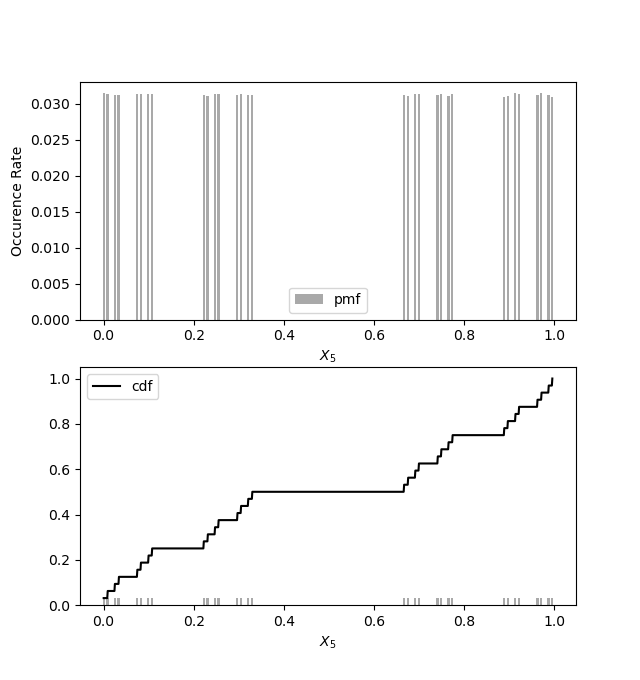
\includegraphics[width=2.5in]{STATS509/HW2/HW2Figures/problem1c.png}
    \end{center}
    \lstinputlisting[language=Python]{HW2Code/HW2_Problem1.py}
\end{enumerate}


\newpage
\section*{Problem 2}
\begin{center}
    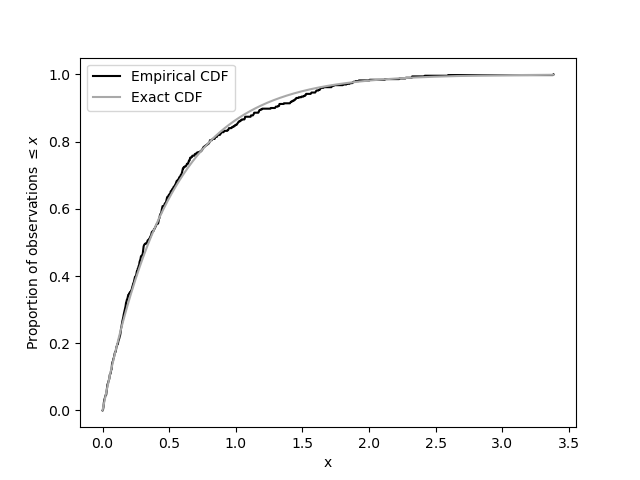
\includegraphics[width=3in]{STATS509/HW2/HW2Figures/problem2.png}
\end{center}
\lstinputlisting[language=Python]{HW2Code/problem2.py}


\newpage
\section*{Problem 3}
\begin{enumerate}
	\item As in all the problems above the empirical CDF is just a counting function:
	$$\F(t) = \frac{1}{n}\sum_{i=1}^n \1\{x_i\leq t\}$$
	
	\item I assume Rectangular distribution is the Uniform distribution given by:
	$$ f(x)=\begin{cases}
            \frac{1}{b - a} & \mathrm{for}\ a \le x \le b, \\
            0 & \mathrm{for}\ x<a\ \mathrm{or}\ x>b
            \end{cases}
    $$
    In this problem we are given that $b=1$ and $a=0$ so that $f(t)=1$ for $0\leq t \leq 1$. CDF, given by the definition $\F(x) = \int f(x) dx$, in this problem is then:
    $$ \F(t) = \int_{-\infty}^{\infty} f(t) dt = 
        \begin{cases}
            0 & \mathrm{for}\ t < 0 \\
            \int_0^tdt = t & \mathrm{for}\ 0 \leq t \leq 1 \\
            1 & \mathrm{for}\  t > 1
        \end{cases}
    $$
    
    \item Code producing this plot can be found at the end of this problem.
    \begin{center}
    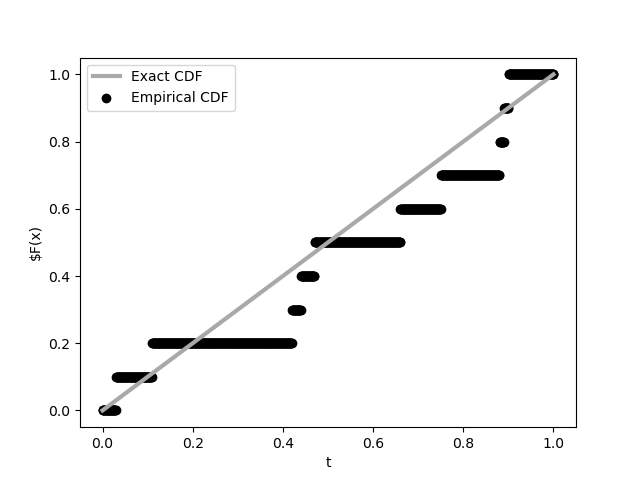
\includegraphics[width=2.5in]{STATS509/HW2/HW2Figures/problem3.png}
    \end{center}
    
    \item Code producing this output can be found at the end of this problem.
    \begin{lstlisting}[language=Python]
        KS statistic K=0.2194194194194194 at point t=0.4194194194194194
    \end{lstlisting}

\newpage
\lstinputlisting[language=Python]{HW2Code/problem2.py}
\end{enumerate}	
	
	
\newpage
\section*{Problem 4}
For each of the following, use the CDF approach to obtain the PDF of Y:
\begin{enumerate}
    \item $Y=2X$ if $X$ is a distributed exponential distribution. The exponential distribution is defined as:
    $$
    F(x;\lambda) = \begin{cases}
                    1-e^{-\lambda x} & x \ge 0, \\
                    0 & x < 0.
                    \end{cases}
    $$
    In a similar manner we can define $G(y)=P(Y\leq y)$ as the CDF of Y. Since CDF is just an integrated PDF we know we can recover the integrand, i.e. the PDF, by deriving $G$. First, since we are given the CDF of X, but not of Y we need to write out the explicit form of $G$:
    \begin{align*}
        G(y) &= P(Y\leq y) = P(2X \leq y) = P(X \leq y/2) = F(y/2) \\
        & = \begin{cases}
            1-e^{-\lambda y/2} & y \ge 0, \\
            0 & y < 0.
           \end{cases}
    \end{align*}
    Deriving case $y\ge 0$ we get:
    \begin{align*}
        g(y) &= \frac{\partial}{\partial y} G(y) = \frac{\partial}{\partial y} \left( 1-e^{-\frac{\lambda y}{2}} \right) \\
             &=  -e^{-\frac{\lambda y}{2}}  \frac{\partial}{\partial y} \left( -\lambda \frac{y}{2} \right) \\
             &= \frac{\lambda}{2} e^{-\frac{\lambda}{2}y}
    \end{align*}
    Finally we note that deriving the case $y,0$ retrieves just $0$. 
    
    \item $Y=-\ln{X}$ if $X$ is a Rectangular on $[0.1]$ I, again, assume Rectangular distribution is the Uniform distribution given by:
	$$ f(x)=\begin{cases}
            \frac{1}{b - a} & \mathrm{for}\ a \le x \le b, \\
            0 & \mathrm{for}\ x<a\ \mathrm{or}\ x>b
            \end{cases}
    $$
    whose CDF we determined in a previous problem as:
     $$ \F(t) = \int_{-\infty}^{\infty} f(t) dt = 
        \begin{cases}
            0 & \mathrm{for}\ t < 0 \\
            t & \mathrm{for}\ 0 \leq t \leq 1 \\
            1 & \mathrm{for}\  t > 1
        \end{cases}
    $$
    Again, write the CDF of $Y$ in terms of $F$ as:
    $$G(y) &= P(Y\leq y) = P(-\ln{X} \leq y) = P(\ln{X} \geq -y) = P(X \geq e^-y)$$
    Here we have to notice the complementarity $P(X\geq a) + P(X< a) = 1$ from which it follows that  $G(y) = 1 - P(X \leq e^{-y}) = 1 - F(e^{-y})$. Finally, we can write 
	$$ G(y)=\begin{cases}
            0& \mathrm{for}\ y \leq 0, \\
            1 - e^{-y} & \mathrm{for}\ y > 0
            \end{cases}
    $$
    Noting that differentiating first case will just produce $0$, we focus on the case $y>0$:
    \begin{align*}
        g(y) &= \frac{\partial}{\partial y} G(y) = \frac{\partial}{\partial y} \left( 1-e^{-y} \right) \\
             &=  e^{-y}
    \end{align*}
    
    \newpage
    \item $Y=X^2$ if X follows normal distribution. Again the trick is to find a clever way to write the CDF $G(y)$. The CDF of normal distribution can not be expressed using elementary functions and is instead given as an integral:
    $$F(x) = \frac 1 {\sqrt{2\pi}} \int_{-\infty}^x e^{-t^2/2} \, dt$$
    We can write $G$ as:
    \begin{align*}
        G(y) &= P(Y\leq y) = P(X^2 \leq y) = \\
             &= P(-\sqrt{y} \leq X \leq \sqrt{y}) \\
             &= P(X \leq \sqrt{y}) - P( X\leq -\sqrt{y}) = F(\sqrt{y}) - F(-\sqrt{y})
    \end{align*}
    Simply because it's just the way it is: 
    \begin{center}
        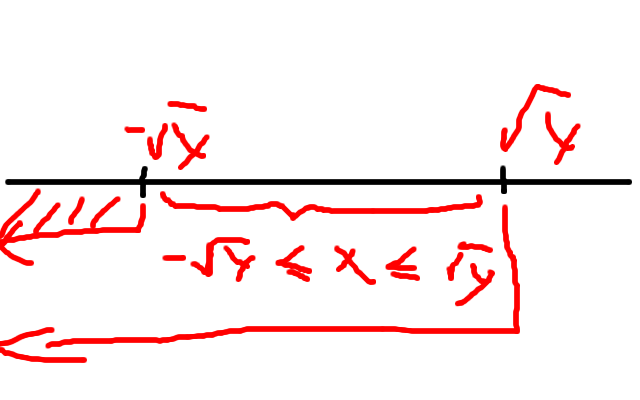
\includegraphics[width=1.5in]{HW2Figures/Picasso.png}
    \end{center}
    In addition to the ways things just are what they are it's also important to remember that the derivative of a CDF is just the PDF: $\partial_x F(x) = f(x)$, i.e. the normal distribution. Finally differentiating the CDF we have:
    \begin{align*}
        g(y) &= \frac{\partial}{\partial y} \left[F(\sqrt y) - F(- \sqrt y) \right] \\
             &=  \frac{\partial \sqrt y }{\partial y} \frac{\partial F(\sqrt y) }{\partial y} - \frac{\partial - \sqrt y}{\partial y} \frac{\partial F(- \sqrt y) }{\partial y} \\
             & = \frac{y^{-1/2}}{2} f(\sqrt y) -  \frac{y^{-1/2}}{2} f(-\sqrt y) \\
    \end{align*}
    Where we just applied the chain rule $\partial_x f(g(x)) = g'(x) f'(g(x))$. Since the normal distribution is symmetric around zero we can say that $f(\sqrt y) = f(-\sqrt y)$, pull the common factors out and simplify:
    $$g(y) = y^{-\frac{1}{2}} f(\sqrt y) = \frac{1}{\sqrt{2\pi y}}e^{-\frac{y}{2}} $$
\end{enumerate}

\newpage
\section*{Problem 5}
The code that produced the following plots is located at the end of the problem.
\begin{enumerate}
    \item 
    \begin{center}
    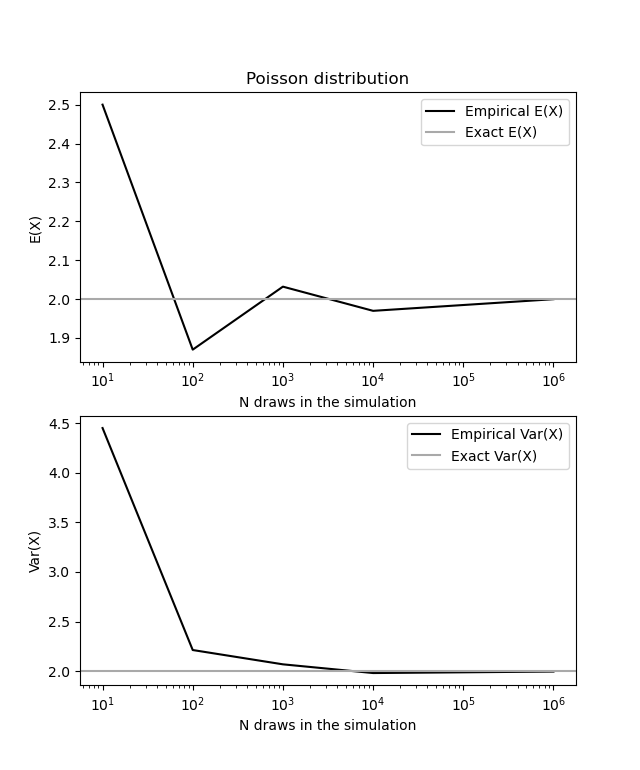
\includegraphics[width=3in]{STATS509/HW2/HW2Figures/problem5a.png}
    \end{center}
     \item 
    \begin{center}
    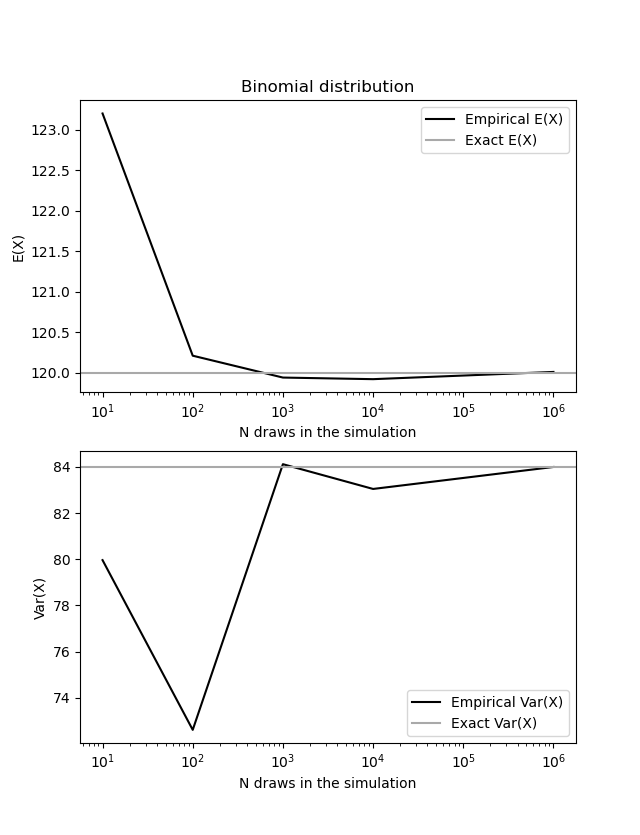
\includegraphics[width=3in]{STATS509/HW2/HW2Figures/problem5b.png}
    \end{center}
\end{enumerate}
\newpage
\lstinputlisting[language=Python]{HW2Code/problem5.py}



\newpage
\section*{Problem 6}
\begin{enumerate}
    \item From hint we know we have to focus on tossing the unfair coin twice. Then we have four possible outcomes $X=\{hh, ht, th, tt\}$. In this sample space the probability of events $ht = p(1-p) = (1-p)p = th$ could be different from 0.5, i.e. for $p=0.2$ the probability of $ht=th=0.2\cdot 0.8=0.16 \neq 0.5$, but the probabilities of $ht$ and $th$ will be equal. However, while individual probabilities $P(ht)$ or $P(th)$ are not 0.5, the probability to get an event from the smaller sample space $P(x|x \in X \cap hh \cap tt) = P(X\in\{ht, th\})$ should be 0.5. I might have mangled the notation a bit, but the point is toss the coin until one gets $ht$ or $th$ outcome, ignoring others. The probability to either get the $ht$ or $th$ in that order are then 50\%. 
    
    \item The probability that in a single toss we first toss a head and then a tail, or first a tail and then a head would be:
    $$P(ht \cup th) = P(ht) + P(th) - P(ht \cap th) = p(1-p) + (1-p)p = 2p(1-p)$$
    Geometric distribution lets us model the number of failures before the first success if all of the trials are mutually independent. The distribution is defined as:
    $P(Y=k) = p(1-p)^k$
    where $k$ is the number of failures before the first success, each with probability $p$. In this case, we do not consider each instance the coin is tossed, but each time we toss it twice. Then probability of each double-toss is given by expression above. So we carefully denote two different $p$'s in these equations by saying $p' = p$ and rewriting:
    $P(Y=k) = p'(1-p')^k$
    The expectation value of the geometric distribution is given as:
    $$E=\frac{1}{p'}$$
    so in our case we can expect to have to toss pairs of coins:
    $$E = \frac{1}{2p(1-p)}$$
    Since the question is potentially confusing, inquiring about the number of times requiring to toss the actual coin not pairs, we can double that expectation value - relying on the linearity of expectation value - to get the actual number of times we had to toss the actual coin and not pairs:
    $$E = \frac{1}{p(1-p)}$$
    
    \item \lstinputlisting[language=Python]{HW2Code/problem6.py}
    
    \item Average number of coin tosses, across 1000 simulations, until success was 6.13. When we climb up to 10 000 simulations I get 6.21 and I get really close to theoretically predicted value of $\frac{1}{0.2\cdot 0.8}=6.25$ with the average value across a million simulations of 6.2501. Now this is the total number of count tosses total, the total number of the $ht$ and $th$ event tosses are then half of that, due to linearity of expectation values we can just move a factor in or out. 
\end{enumerate}


\newpage
\section*{Problem 7}
For each of the following distribution calculate expectation value and variance. Expressions taken from Goldberger table 3.1.
\begin{enumerate}
    \item Discrete uniform with N=9
    \begin{align*}
        E(X) &= \frac{N+1}{2} = 5 \\
        V(X) &= \frac{N^2-1}{12} = 6.666...
    \end{align*}
    
    \item Binomial with n=2 and p=0.4
    \begin{align*}
    E(X) &= np = 0.8 \\
    V(X) &= np(1-p) = 0.48
    \end{align*}
    
    \item Binomial with n=4 and p=0.6
    \begin{align*}
    E(X) &= np = 2.4 \\
    V(X) &= np(1-p) = 0.96
    \end{align*}
    
    \item Poisson with $\lambda=2$
    \begin{align*}
    E(X) &= \lambda = 1.5 \\
    V(X) &= \lambda = 1.5
    \end{align*}
    
    \item Rectangular on $[0,2]$ (again, assuming uniform)
    \begin{align*}
    E(X) &= \frac{a+b}{2} = 1 \\
    V(X) &= \frac{(b-a)^2}{12} = 0.333
    \end{align*}

    \item Exponential with $\lambda=2$
    \begin{align*}
    E(X) &= \frac{1}{\lambda} = 0.5 \\
    V(X) &= \frac{1}{\lambda^2} = 0.25
    \end{align*}
    
    \item Powerlaw with $\theta=2$ on $[0,1]$
    \begin{align*}
    E(X) &= \theta/(1+\theta) = 0.75 \\
    V(X) &= \theta\left[ (1+\theta)^2(2+\theta)\right]^{-1} = 0.0555...
    \end{align*}
\end{enumerate}


\end{document}
